\documentclass[11pt]{article}
\usepackage[top=1.5cm,bottom=1.5cm,left=1.5cm,right= 1.5cm]{geometry}
%\geometry{landscape}                % Activate for for rotated page geometry
\usepackage[parfill]{parskip}    % Activate to begin paragraphs with an empty line rather than an indent
\usepackage{graphicx}
\usepackage{amssymb}
\usepackage{epstopdf}
\usepackage{setspace}            
\usepackage{amsmath}            
\usepackage{multirow}    
\usepackage{changepage}
\usepackage{lscape}
\usepackage{ulem}
\usepackage{multicol}
\usepackage{dashrule}
\usepackage[usenames,dvipsnames]{color}       
\usepackage{enumerate}
\newcommand{\urlwofont}[1]{\urlstyle{same}\url{#1}}
\newcommand{\degree}{\ensuremath{^\circ}}

\DeclareGraphicsRule{.tif}{png}{.png}{`convert #1 `dirname #1`/`basename #1 .tif`.png}

\newenvironment{choices}{
\begin{enumerate}[(a)]
}{\end{enumerate}}

\pagestyle{empty}

%\newcommand{\soln}[1]{\textcolor{MidnightBlue}{\textit{#1}}}	% delete #1 to get rid of solutions for handouts
\newcommand{\soln}[1]{ \vspace{2.7cm} }

\newcommand{\solnMult}[1]{\textbf{\textcolor{MidnightBlue}{\textit{#1}}}}	% uncomment for solutions
%\newcommand{\solnMult}[1]{ #1 }	% uncomment for handouts

%\newcommand{\pts}[1]{ \textbf{{\footnotesize \textcolor{black}{(#1)}}} }	% uncomment for handouts
\newcommand{\pts}[1]{ \textbf{{\footnotesize \textcolor{red}{(#1)}}} }	% uncomment for handouts

\newcommand{\note}[1]{ \textbf{\textcolor{red}{[#1]}} }	% uncomment for handouts

\definecolor{oiG}{rgb}{.298,.447,.114}
\definecolor{oiB}{rgb}{.337,.608,.741}

\usepackage[colorlinks=false,pdfborder={0 0 0},urlcolor= oiG,colorlinks=true,linkcolor= oiG, citecolor= oiG,backref=true]{hyperref}

%\usepackage{draftwatermark}
%\SetWatermarkScale{4}

\usepackage{titlesec}
\titleformat{\section}
{\color{oiB}\normalfont\Large\bfseries}
{\color{oiB}\thesection}{1em}{}
\titleformat{\subsection}
{\color{oiB}\normalfont}
{\color{oiB}\thesubsection}{1em}{}

\newcommand{\ttl}[1]{ \textsc{{\LARGE \textbf{{\color{oiB} #1} } }}}

\newcommand{\tl}[1]{ \textsc{{\large \textbf{{\color{oiB} #1} } }}}

\begin{document}

Dr. \c{C}etinkaya-Rundel \hfill Data Analysis and Statistical Inference \\

\ttl{Application exercise: \\
4.1 Bootstrap intervals} 

\section*{Comedies on RottenTomatoes}

The following histogram shows the distribution of RottenTomatoes scores of a random sample of 54 comedies. The average score is 52.52 (out of 100).

\begin{center}
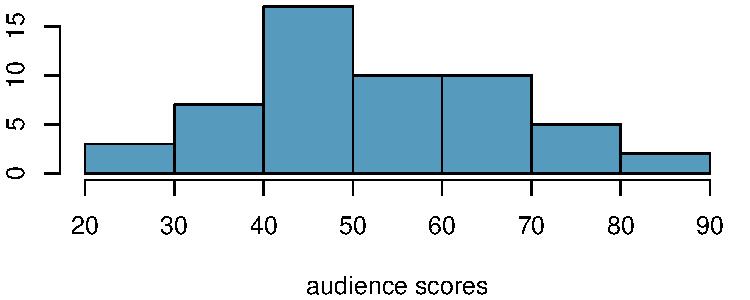
\includegraphics[width = 0.7\textwidth]{figures/comedy_hist}
\end{center}

The dot plot below shows the distribution of 200 bootstrap means calculated based on this sample.

\begin{center}
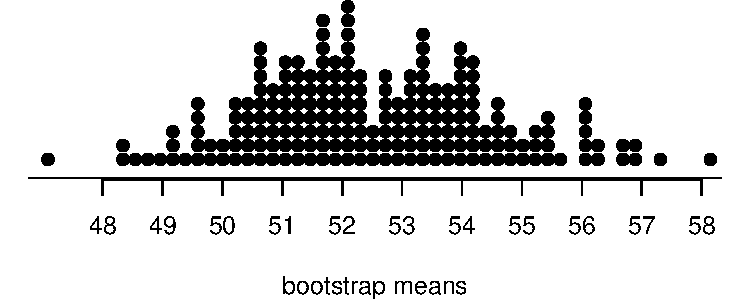
\includegraphics[width = 0.7\textwidth]{figures/comedy_boot_mean_dot}
\end{center}

The mean of the bootstrap distribution is 52.5, and the bootstrap standard error is  1.98.

\begin{enumerate}

\item Describe in detail how this bootstrap distribution is constructed, outlining each step.

\item Construct a 95\% bootstrap interval for the average RottenTomatoes score of comedies, using both methods.

\item Describe the differences and similarities between bootstrap and sampling distributions.

\end{enumerate}




%

\end{document}